	\subsection{Objetivos}

		En este informe se busca aplicar los conocimientos adquiridos durante la visita al Laboratorio de Acústica y Luminotecnia, en donde se realizaron ciertas experiencias con la cámara reverberante, la cámara anecoica y el tubo de Kundt. En particular, el objetivo consta en caracterizar unas pantallas que se desean instalar en un proyecto real, por lo que se realizará el análisis adecuado para saber si cumplen con las características requeridas.
		
	\subsection{Especificaciones}
	
	El proyecto del viaducto del ramal Retiro-Tigre del tren Mitre requiere instalar unas pantallas que deben tener las siguientes características acústicas:
		
		\begin{table}[h!]
			\centering
			\begin{tabular}{ccc}
			\toprule
			\textbf{Característica} & \textbf{Requerimiento} & \textbf{Normativa de aplicación}\\
			\midrule
			Aislamiento al ruido aéreo & Categoría B3 & UNE-EN $1793$-$2$:$2014$, Anexo A\\
			Absorción sonora & Categoría A3 & UNE-EN $1793$-$2$:$2014$, Anexo A\\
			\bottomrule
			\end{tabular}
		\end{table}
		
	\subsection{Descripción de la muestra ensayada}
		
		Se ensayaron módulos para construcción de barreras acústicas construidos con paneles \textit{tipo sándwich}, conformados por una chapa de acero galvanizado (ciega), una capa de lana de roca y una chapa de acero galvanizado perforada (densidad de perforación del $40\%$). La superficie de la muestra era de \SI{10}{\square\meter}.\\
		
		Las pantallas instaladas a lo largo del viaducto del tren Mitre quedarían de la siguiente manera:

		\begin{figure}[H]
			\centering
		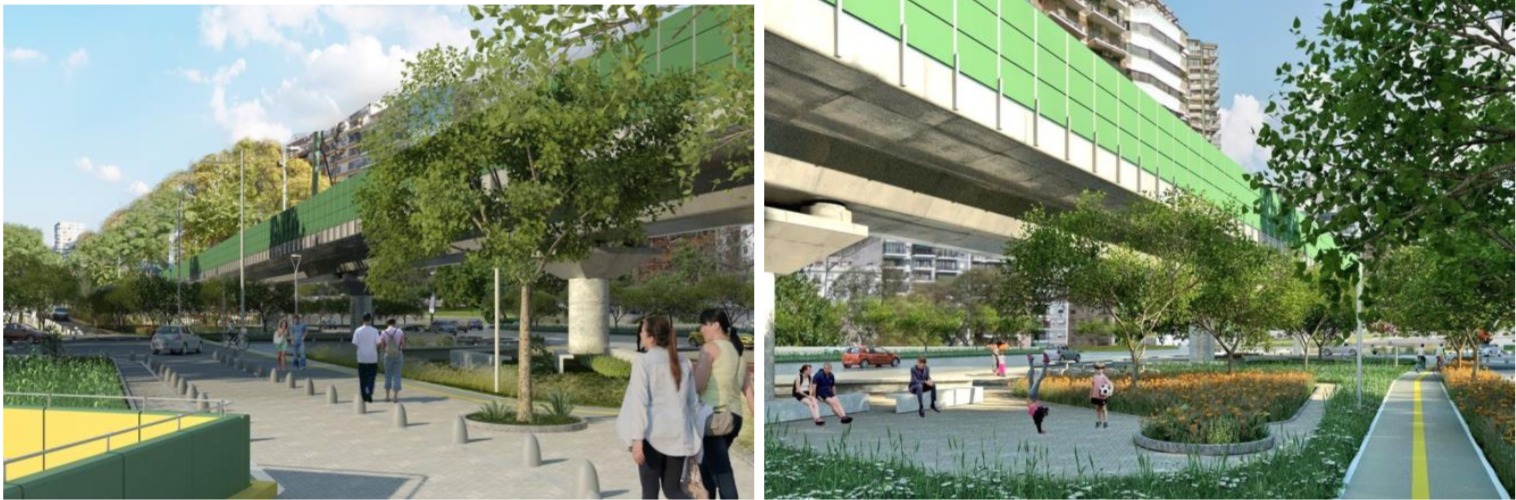
\includegraphics[scale=0.50]{intro_vistas.png}\\
			\caption{Vistas de las barreras acústicas a colocar en el viaducto del Tren Mitre.}
			\label{intro_vistas}
		\end{figure}
